\documentclass[12pt,twoside]{article}
\usepackage{amsmath, amssymb}
\usepackage{amsmath}
\usepackage[active]{srcltx}
\usepackage{amssymb}
\usepackage{amscd}
\usepackage{makeidx}
\usepackage{amsthm}
\usepackage{algpseudocode}
\usepackage{algorithm}
\usepackage{graphicx}
\usepackage[spanish]{babel}
\renewcommand{\baselinestretch}{1}
\graphicspath{{images/}}
\setcounter{page}{1}
\setlength{\textheight}{21.6cm}
\setlength{\textwidth}{14cm}
\setlength{\oddsidemargin}{1cm}
\setlength{\evensidemargin}{1cm}
\pagestyle{myheadings}
\thispagestyle{empty}
\markboth{\small{Pr\'actica 3. Alan, Josu\'e}}{\small{.}}
\date{}
\begin{document}
\centerline{\bf An\'alisis de Algoritmos, Sem: 2020-1, 3CV2, Pr\'actica 2, 28 de agosto}
\centerline{}
\centerline{}
\begin{center}
\Large{\textsc{Pr\'actica 3: Divide y venceras, algoritmo MergeSort}}
\end{center}
\centerline{}
\centerline{\bf {Alan Romero Lucero, Josué David Hern\'andez Ram\'irez}}
\centerline{}
\centerline{Escuela Superior de C\'omputo}
\centerline{Instituto Polit\'ecnico Nacional, M\'exico}
\centerline{$alanrl.escom@gmail.com, correo@alumno_2$}
\newtheorem{Theorem}{\quad Theorem}[section]
\newtheorem{Definition}[Theorem]{\quad Definition}
\newtheorem{Corollary}[Theorem]{\quad Corollary}
\newtheorem{Lemma}[Theorem]{\quad Lemma}
\newtheorem{Example}[Theorem]{\quad Example}
\bigskip
\textbf{Resumen:} La presente pr\'actica muestra la implementaci\'on del algoritmo de ordenamiento \textit{MergeSort}, el cual funciona bajo el principio de divide y venceras.
{\bf Palabras Clave:} {\textit{algoritmo, ordenamiento, $big O$, merge sort}}
\section{Introducci\'on}
De entre todos los algoritmos que existen, podemos decir que los algoritmos de ordenamiento son algunos de los m\'as cl\'asicos por analizar cuando se est\'a estudiando. Eso no es simplemente por que sean muy divertidos, sino por el dolor de cabeza que representan y su importancia en la actualidad. En la era de informaci\'on el poder odernar datos se vuelve muy habitual y necesario, raz\'on por lo que estos algoritmos son constantement estudiados y analizados.

De entre la gran cantidad de algoritmos famosos de ordenamiento, se suelen destacar los mas complejos y lentos, como el \textit{BubleSort} o el \textit{BogoSort}, as\'i como los menos complejos y con muy buenos tiempos de ejecuci\'on como los son el \textit{QuickSort} o el \textit{MergeSort}. De este \'ultimo, analizaremos y veremos su complejidad, adem\'as del algoritmo que hace posible su funcionamiento, el algoritmo de \textit{Merge}.

\section{Conceptos B\'asicos}
El \textit{MergeSort} trabajo bajo el principio b\'asico de divide y venceras. Este famoso dicho plantea que un problema grande puede ser resuelto si se divide en muchos problemas muy pequeño, as\'i como faciles de resolver. Dicho el algorimo funciona de la siguiente manera:
\begin{itemize}
    \item Si la lista es de tamño uno o menor, no se hacen nada
    \item Dada una lista de tamaño $n$, se divide aproximadamente por la mitad en dos listas del mismo tamaño.
    \item Posteriormente se aplica el mismo algoritmo a ambas listas nuevas de tamaño $\frac{n}{2}$.
    \item Finalmente de unen ordenadamente ambas listas con el algoritmo de \textit{Merge}
\end{itemize}
Pasando esto a pseudoc\'odigo:
\begin{center}
    \begin{algorithmic}[1]
        \Procedure{MergeSort}{lista=$[A\textsubscript{1}, \dots, A\textsubscript{len}]$}
            \If{$len > 1$}
                \State $med \longleftarrow \frac{len}{2}$
                \State $primerMitad \longleftarrow MergeSort([A\textsubscript{1}, \dots, A\textsubscript{med}])$
                \State $segundaMitad \longleftarrow MergeSort([A\textsubscript{med+1}, \dots, A\textsubscript{len}])$
                \State \textbf{return} $Merge(primerMitad, segundaMitad)$
            \EndIf
        \EndProcedure
    \end{algorithmic}
\end{center}
Visto esto, hace falta definir como es que el algoritmo \textit{Merge} ordena las lista que recibe, el cual termina haciendo tan efectivo al \textit{MergeSort} que simplementa divide la lista de manera recursiva. El \textit{Merge} se hace de la siguiente manera: 
\begin{center}
    \begin{algorithmic}[1]
        \Procedure{Merge}{listaUno = $[A\textsubscript{1},\dots,A\textsubscript{n}],$,listaDos = $[B\textsubscript{1}, \dots, B\textsubscript{m}]$}
            \State $i \longleftarrow 0$
            \State $j \longleftarrow 0$
            \State $resultado \longleftarrow []$
            \While{$i<n$ \textbf{and} $j<m$}
                \If{$A\textsubscript{i} < B\textsubscript{j}$}
                    \State $resultado$ append $A\textsubscript{i}$
                    \State $i \longleftarrow i + 1$
                \Else
                    \State $resultado$ append $B\textsubscript{j}$
                    \State $j \longleftarrow j + 1$
                \EndIf
            \EndWhile
            \If{$n < m$}
                \State $resultado$ append $[B\textsubscript{j}, \dots, B\textsubscript{m}]$
            \Else
                \State $resultado$ append $[A\textsubscript{j}, \dots, A\textsubscript{n}]$
            \EndIf
            \State \textbf{return} $resultado$
        \EndProcedure
    \end{algorithmic}
\end{center}
Analicemos ahora el algoritmo merge. Analizando por bloques, se enlistan el rango de las lineas de los bloques y su complejidad.
\begin{figure}[ht]
    \centering
    \begin{equation}
        linea[2-4] \in \mathcal{O}(c)
    \end{equation}
    \begin{equation}
        linea[6-11] \in \mathcal{O}(c)
    \end{equation}
    \begin{equation}
        linea[5-13] \in \mathcal{O}(n)
    \end{equation}
    \begin{equation}
        linea[14-19] \in \mathcal{O}(c)
    \end{equation}
    \caption{Analisis por bloques del algoritmo \textit{Merge}}
    \label{sec:analisis}
\end{figure}
Se puede ver que de las lineas 5 a 11 estan contenidas en el bloque while, el cual comprende de las lineas 5 a la 13. Entonces tenemos en el mismo nivel bloque de complejidad $\mathcal{O}(1)$ y una de complejidad $\mathcal{O}(n)$. Por los teoremas vistos en clase, nos quedamos con la complejidad $\mathcal{O}(n)$. Para terminar, podemos decir que $\textit{Merge} \in \mathcal{O}(n)$.

Una vez analizado el algoritmo de \textit{Merge}, analicemos el algoritmo del \textit{MergeSort}. Para esto se tiene que plantear una ecuacion de recurrencia, siendo $n$ la longitud de la lista.
\[
    T(n) = 
\begin{cases}
    c, & \text{si } n \leq 1 \\
    2T(\frac{n}{2}) + bn, & n > 1
\end{cases}
\]
La funcion queda asi, debido que a si la lista es muy pequeña, de longitud $n$ 1 o 0 el algoritmo ya no hace nada, pero hace la comparacion por lo que se la asigna una constante c. Ahora, cuando $n$ es mayor a uno, entonces el merge se ejecuta a s\'i mismos dos veces, por la primer y segunda mitad de la lista original. Dentro de ese mismo bloque se realiza el algoritmo \textit{Merge}, el cual como ya se demostr\'o anteriormente, tiene complejidad $\mathcal{O}(n)$. Se reescribira la ecuaci\'on mediante una variable $k = \log_{2} n$
\[
    T(2\textsuperscript{k}) = 
\begin{cases}
    c, & \text{si } k = 0 \\
    2T(2\textsuperscript{k-1}) + 2\textsuperscript{k}, & k > 0
\end{cases}
\]
Ahora, se desarrollar\'a la ecuacion de recurrencia, obteniendo como resultado que $\textit{MergeSort} \in \mathcal{O}(n*\log_{2} n)$.
\begin{figure}[ht]
    \centering
    \begin{equation}
        T(2\textsuperscript{k}) = 2*T(2\textsuperscript{k-1})+2\textsuperscript{k}
    \end{equation}
    \begin{equation}
        =2*(2*T(2\textsuperscript{k-2}) + 2\textsuperscript{k}) + 2\textsuperscript{k}
    \end{equation}
    \begin{equation}
        =2\textsuperscript{2}*T(2\textsuperscript{k-2})+2*2\textsuperscript{k}
    \end{equation}
    \begin{equation}
        = \dots
    \end{equation}
    \begin{equation}
        =2\textsuperscript{i}*T(2\textsuperscript{k-i})+i*2\textsuperscript{k}
    \end{equation}
    \begin{equation}
        \dots
    \end{equation}
    \begin{equation}
        k-i = 0 \longrightarrow i = k
    \end{equation}
    \begin{equation}
        \dots
    \end{equation}
    \begin{equation}
        =2\textsuperscript{k}*T(2\textsuperscript{k-k})+k*2\textsuperscript{k}
    \end{equation}
    \begin{equation}
        =2\textsuperscript{k}T(1)+k*2\textsuperscript{k}
    \end{equation}
    \begin{equation}
        =c*2\textsuperscript{k}+k*2\textsuperscript{k}
    \end{equation}
    \begin{equation}
        \text{\textit{recordando }} k = \log_{2} n
    \end{equation}
    \begin{equation}
        =c*n+n*\log_{2} n
    \end{equation}
    \begin{equation}
        \text{\textit{entonces }} T(n) \in \mathcal{O}(c*n + n*\log_{2} n)
    \end{equation}
    \begin{equation}
        \text{\textit{finalmente, simplificando }} T(n) \in \mathcal{O}(n*\log_{2} n)
    \end{equation}
    \caption{Desarrollo de la ecuaci\'on de recurrencia}
    \label{eq:desarrollo_recurrencia}
\end{figure}

\newpage
\vfill
\clearpage
\section{Experimentaci\'on y Resultados}
La implementaci\'on de los algoritmos merge y merge-sort fueron probadas con datos aleatorios.
\subsection{Merge}
Para comprender de mejor manera como actua el algoritmo de Merge, se procedió a realizar una grafica de su complejidad para que de esta manera se entienda que su complejidad es lineal.
\begin{figure}{ht}
    \centering
    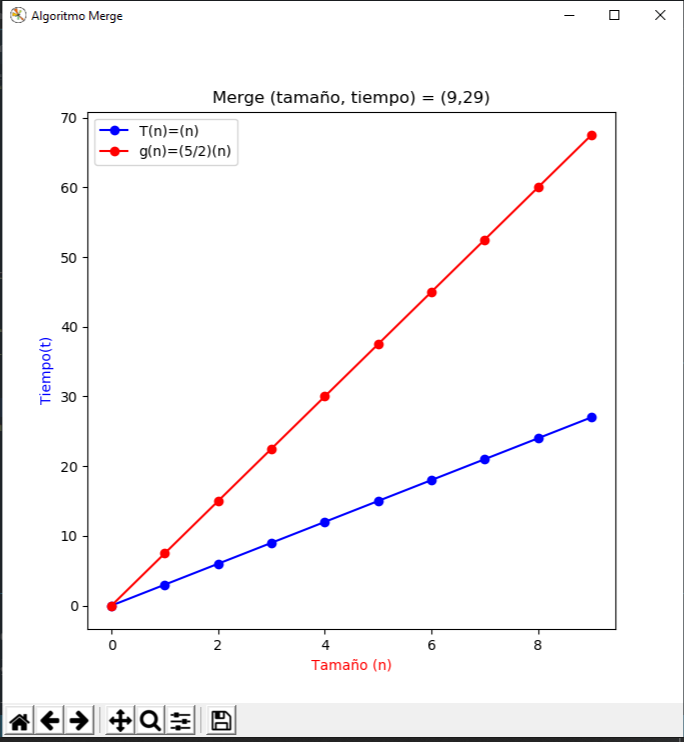
\includegraphics[width=13cm, height=10cm]{merge-graph.png}
    \caption{Gr\'afica del algoritmo Merge}
    \label{fig:merge_graph}
\end{figure}


\begin{figure}{ht}
    \centering
    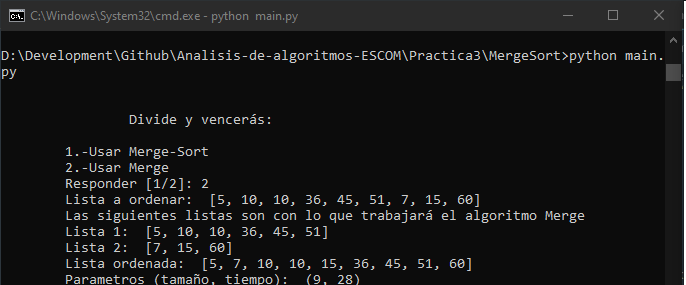
\includegraphics[width=13cm, height=6cm]{merge-program.png}
    \caption{Programa del algoritmo Merge}
    \label{fig:merge_program}
\end{figure}

\subsection{Merge-Sort}
Por otro lado el algoritmo de Merge-Sort tiende a ser \begin{equation}
    =c*n+n*\log_{2} n
\end{equation} aunque de manera experimental esto no se pueda apreciar, debido a la cantidad de datos aleatorios probados y por ende, al ser aleatorios puede estar la probabilidad de que estos datos se repitan o puedan estar ordenados.
\begin{figure}{ht}
    \centering
    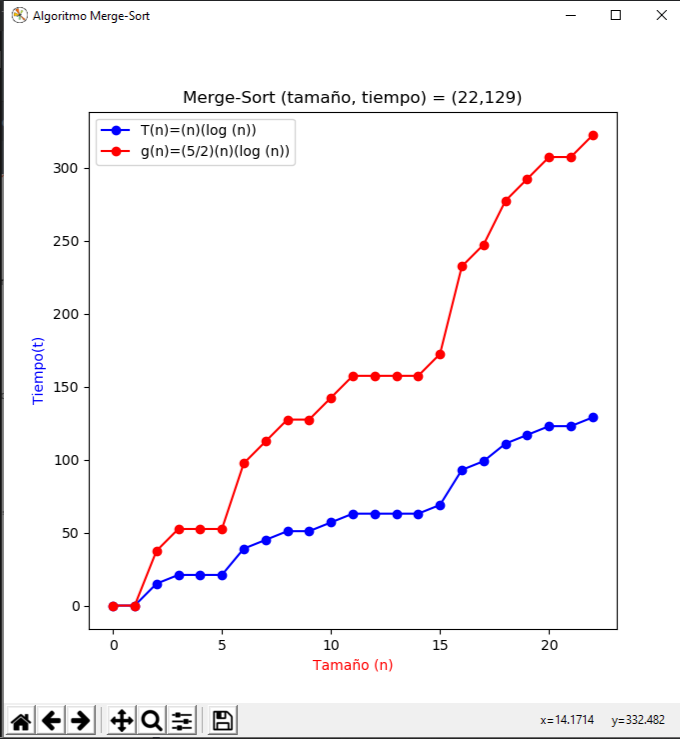
\includegraphics[width=13cm, height=10cm]{mergesort-graph.png}
    \caption{Gr\'afica del algoritmo Merge}
    \label{fig:mergesort_graph}
\end{figure}


\begin{figure}{ht}
    \centering
    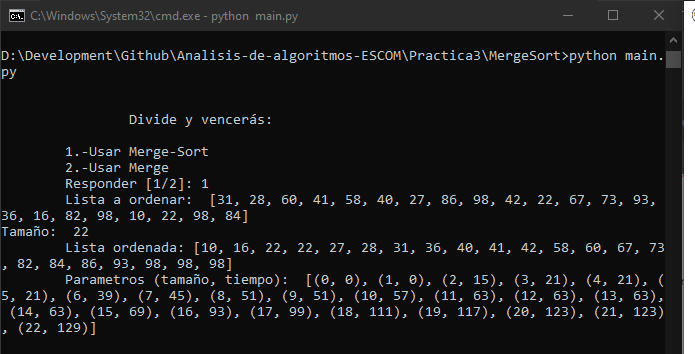
\includegraphics[width=13cm, height=6cm]{mergesort-program.png}
    \caption{Programa del algoritmo Merge}
    \label{fig:mergesort_program}
\end{figure}

\section{Conclusiones}



\textit{Alan Romero Lucero}. En esta pr\'actica ya calculamos la complejidad de un algoritmo recursivo de una manera mas formal, mediante la ecuacion de recurrencia. El merge sort es interesante, sobre todo por su complejidad bastante baja y buena para un algoritmo de ordenamiento, y es interesante como ayuda dividir el problema en problemas de menor complejidad. En este caso, reduce el problema al dividir la lista hasta dos listas que estan ordenadas, para finalmente mezclarlas con un algoritmo de complejidad lineal, el \textit{Merge}.


\textit{Josu\'e David Hern\'andez Ram\'irez}. Esta pr\'actica ha sido de las m\'as tediosas, puesto que al tener funciones que se madnan a llamar el contador para calcular el tiempo que lleva el algoritmo en concretarse se llega perder su valor en la fase de programación. Las ventajas que tienen estos algoritmos es su complejidad, puesto que al no ser tan alta, este puede concretarse en menos tiempo lo que beneficia al usuario al implementarlo. El algoritmo de merge es el primer paso para poder crear el algoritmo de merge, ya que este, se puede decir que hace el "trabajo sucio" de ordenar, pero lo que necesita para funcionar correctamente es que las dos listas que necesita para trabajar deben de estar previamente ordenadas para que el algoritmo funcione eficazmente.

Para esto, se crea su complemento ya que, en teoría, el merge puede dividr la lista en 2 con igual o menor tamaño respecto a la otra, lo que conlleva a que tarde mas en concretarse, para esto el Merge Sort se encarga de leer una lista y este la divide exactamente en dos y asi sucesivamente en ambas partes hasta que todos los elementos de la lista estan solos, cuando esto pase, procede a ordenar los elementos del menor al mayor.\textit{Merge}.
 
\newpage
\vfill
\clearpage
\section{Anexo}
En la pr\'actica se proporcionan dos algoritmos, A y B, de los cuales se tiene que calcular su complejidad aplicando lo visto en clase.
\begin{figure}[ht]
    \centering
    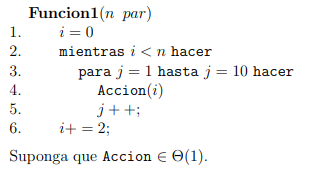
\includegraphics{anexo_uno.png}
    \caption{Algoritmo A planteado en la pr\'actica}
    \label{fig:algoritmo_a}
\end{figure}
Para el primer bloques, al hacer el analisis por bloques se tiene los siguiente: el bloque de instrucciones de las lineas 4-5 son $\mathcal{O}(c) \longrightarrow  \mathcal{O}(1)$, se encuentran dentro de un for, pero el for tiene un numero fijo independiente al n pasado como argumento, por lo que su complejidad tambien es constante, $\mathcal{O}(c)$. Finalmente, al mismo nivel se encuntra un bloque de complejidad $\mathcal{O}(1)$ y un ciclo while de complejidad $\mathcal{O}(n)$. En el caso de este algoritmo, tanto para el mejor como para el peor caso la complejidad no cambia, dado que el bloque while se ejecuta siempre $cn$ veces y los bloques internos no son dependientes del $n$ pasado a la funcion. Por lo anterior $\Omega (n) = \mathcal{O}(n)  \longleftarrow  Funcion1 \in \Theta(n)$.

\begin{figure}[ht]
    \centering
    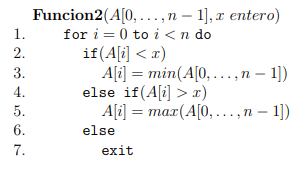
\includegraphics{anexo_dos.png}
    \caption{Algoritmo B planteado en la pr\'actica}
    \label{fig:algoritmo_b}
\end{figure}

El segundo algoritmo tiene en el nivel mas interno una llamada a la function $min([A\textsubscript{0}, ..., A\textsubscript{n-1}])$ o $max([A\textsubscript{0}, ..., A\textsubscript{n-1}])$. No se dice explicitamente que hacen las funciones o su complejidad, sin embargo se consideraran funciones que buscan el valor minimo y maximo en el arreglo que recibe, por lo que se considera una complejidad $\mathcal{O}(n)$ y $\Omega (1)$. El cuerpo del for tiene complejidad $\mathcal{O}(n)$ y $\Omega (1)$, dado que el if solo va a ejecutar una funcion entra la min o max, el else se analizar\'a mas adelante. Finalmente se encuentra un bucle for de complejidad $\mathcal{O}(n)$ en el peor de los casos cuando el elemento $A\textsubscript{n-1} = x$, sin embargo tiene una complejidad $\Omega(1)$ en el caso en el que $A\textsubscript{0} = x$. En el mejor de los casos, se tiene un bloque de complejidad 1 con un bloque interno de complejidad 1, por lo que la complejidad final del bloque ser\'ia $Funcion2 \in \Omega(1)$. Para el peor casos, se tiene un bloque de complejidad $\mathcal{O}(n)$ que tiene internamente un bloque de complejidad $\mathcal{O}(n)$, por lo que en el peor de los casos su complejidad ser\'ia $\mathcal{O}(n^2)$.

\section{Bibliograf\'ia}
"Merge y MergeSort", class notes for An\'alisis de Algoritmos, ESCOM-IPN, Verano 2019.
\end{document}